%%%%%%%%%%%%%%%%%%%%%%%%%%%%%%%%%%%%%%%%%
% University Assignment Title Page 
% LaTeX Template
% Version 1.0 (27/12/12)
%
% This template has been downloaded from:
% http://www.LaTeXTemplates.com
%
% Original author:
% WikiBooks (http://en.wikibooks.org/wiki/LaTeX/Title_Creation)
%
% License:
% CC BY-NC-SA 3.0 (http://creativecommons.org/licenses/by-nc-sa/3.0/)
% 
% Instructions for using this template:
% This title page is capable of being compiled as is. This is not useful for 
% including it in another document. To do this, you have two options: 
%
% 1) Copy/paste everything between \begin{document} and \end{document} 
% starting at \begin{titlepage} and paste this into another LaTeX file where you 
% want your title page.
% OR
% 2) Remove everything outside the \begin{titlepage} and \end{titlepage} and 
% move this file to the same directory as the LaTeX file you wish to add it to. 
% Then add \input{./title_page_1.tex} to your LaTeX file where you want your
% title page.
%
%%%%%%%%%%%%%%%%%%%%%%%%%%%%%%%%%%%%%%%%%
%\title{Title page with logo}
%----------------------------------------------------------------------------------------
%	PACKAGES AND OTHER DOCUMENT CONFIGURATIONS
%----------------------------------------------------------------------------------------

\documentclass[10pt,technote]{IEEEtran}
\usepackage[english]{babel}
\usepackage[utf8x]{inputenc}
\usepackage{amsmath}
\usepackage{graphicx}
\usepackage{float}
\usepackage[colorinlistoftodos]{todonotes}

\begin{document}

\newcommand{\HRule}{\rule{\linewidth}{0.5mm}} % Defines a new command for the horizontal lines, change thickness here

\begin{center} % Center everything on the page
 
%----------------------------------------------------------------------------------------
%	HEADING SECTIONS
%----------------------------------------------------------------------------------------

\textsc{\small Università degli studi di Milano-Bicocca}\\[1cm] % Name of your university/college
\textsc{\Large Data and Text Mining }\\[0.3cm] % Major heading such as course name
\textsc{Final Project, June 2020}\\[0.1cm] % Minor heading such as course title

%----------------------------------------------------------------------------------------
%	TITLE SECTION
%----------------------------------------------------------------------------------------

\HRule \\[0.6cm]
{ \huge Cervical cancer exploratory study}\\ % Title of your document
\HRule \\[1.0cm]
 
%----------------------------------------------------------------------------------------
%	AUTHOR SECTION
%----------------------------------------------------------------------------------------

\large
\emph{Author:}\\
Antonio Vivace - 793509 a.vivace1@campus.unimib.it \\[1cm] % Your name

\end{center}

\begin{abstract}
The ABSTRACT is not a part of the body of the report itself. Rather, the abstract is a brief summary of the report contents that is often separately circulated so potential readers can decide whether to read the report. The abstract should very concisely summarize the whole report: why it was written, what was discovered or developed, and what is claimed to be the significance of the effort. The abstract does not include figures or tables, and only the most significant numerical values or results should be given.
\end{abstract}

\section{Introduction}

This year in the US, there will be an estimated 13800 new cases of Cervical cancer. 4290 will be deadly \cite{acs}.
Worldwide, this type of cancer causes makes up 8\% of the total cancer cases and deaths. It's the fourth cause of death from cancer in women, with 260 000 deaths in 2012.
A lot of progress has been made, and nowadays it is one of the most treatable: when diagnosed and treated at the earliest stage, the five-year survival rate can reach 95\% \cite{cruk}.

\paragraph{Known causal relations}

HPV causal relation with the cervical cancer has been documented beyond reasonable doubt \cite{Bosch2002}. Additionally, Human papilloma virus (HPV) infection is necessary for the development of CIN, the abnormal growth of cells on the surface of the cervix, indicating a potentially precancerous transformation of cells of the cervix \cite{kumar2017robbins}.

Other risk factors include smoking \cite{Collins2010} early age at the first sexual intercourse and early pregnancies (these two values are also strongly interrelated in most developing countries) \cite{Louie2009}.

\section{Dataset}

The dataset was collected at 'Hospital Universitario de Caracas' in Caracas, Venezuela. The dataset comprises demographic information, habits, and historic medical records of 858 patients.

The missing values are due to the decision of the patients to not disclose those details because of privacy concerns.

Attributes describe patients’ sexual activity and frequency, age, smoke addiction, usage of contraceptives and diagnosed Sexualy Transmitted Diseases.

We'll introduce some context and clarifications on the attributes significance to outline the relationship between the phenomena described:
\begin{enumerate}
    \item \textbf{Hormonal Contraceptives} indicates if the patient uses \textit{hormonal} contraceptives. \textbf{IUD} indicates the usage of the Intra Uterine contraceptive Device.
    \item \textbf{STDs} indicates if the patient had at least one Sexually Transmitted Disease. It's 1 when at least one of the STDs:condylomatosis, STDs:cervical condylomatosis, STDs:vaginal condylomatosis, STDs:vulvo-perineal condylomatosis, STDs:syphilis, STDs:pelvic inflammatory disease, STDs:genital herpes, STDs:molluscum contagiosum, STDs:AIDS, STDs:HIV, STDs:Hepatitis, STDs:HPV variables, is positive.
    \item \textbf{STDs:HPV} indicates if the patient was infected by \textit{Human Papilloma Virus}.
    \item \textbf{Dx:HPV} reveals if the patient was already diagnosed with HPV in the past.
    \item \textbf{Dx:Cancer} is positive if the patient already had cancer. It is not clear if this refers to Breast Cancer, as diagnosable by the Oncotype DX test or any type of cancer. The original paper presenting this dataset has no additional information on this \cite{articleUCI}.
    \item \textbf{Dx:CIN} indicates if the patient was affected by Cervical intraepithelial neoplasia (CIN).
    \item \textbf{Dx} is positive if at least one of the Dx variables is positive.
    \item \textbf{Hinselmann}, \textbf{Citology} are two (complementary \cite{Duncan2004}) tests to detect Cervical Cancer. \textbf{Schiller} is another test able to identify abnormal areas to be biopsied and examined.
    \item \textbf{Biopsy}, our target variable, diagnosing or not the disease.
\end{enumerate}

\section{The Methodological Approach}

\subsection{Exploration}
\begin{figure}
    \centerline{
        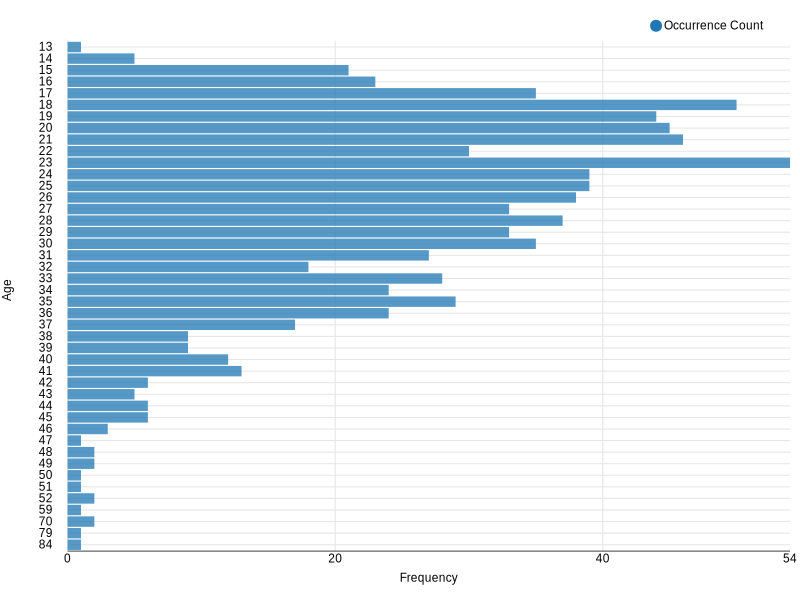
\includegraphics[width=0.4\paperwidth]{figures/age_dist.png}}
    \caption{Age distribution}
    \label{age_distribution}
\end{figure}

\begin{figure}
    \centerline{
        \includegraphics[width=0.3\paperwidth]{figures/class_unbalance.png}}
    \caption{Unbalanced biopsy distribution}
    \label{unbalanced_biopsy}
\end{figure}



The target class is highly unbalanced (Figure \ref{unbalanced_biopsy}), with only 6.4\% of positive values.
The main statistical descriptors have been computed and studied (Figure \ref{numeric_attributes_statistics}). Age distribution is shown in Figure \ref{age_distribution}: the majority of the instances refers to young womans (younger than 15 and older than 38 years old can be considered outliers). Almost all of them had at least one pregnancy (98,1\%).
\subsection{Missing Values}


\subsection{Correlation}

In this step, we aim to expose relations among variables. There a lot of attributes which information is included in other ones, and many other not linked with the target attribute, we want to proceed filtering those out (feature selection).

Some mentioned causal relations can be seen through this step: early age at first sexual intercourse, number of partners.

\textbf{Dx} is not clearly correlated with Biopsy, probably because the type of cancer it refers to it's unrelated (Breast).

Even if it's been shown that smoking it's a risk factor for CIN, the potential initial step of a Cervical Cancer, this is not visibile in this dataset.


\subsection{Class imbalance}
\subsection{Classification}

This is the central and most important section of the report. Its objective must be to show, with linearity and clarity, the steps that have led to the definition of a decision model. The description of the working hypotheses, confirmed or denied, can be found in this section together with the description of the subsequent refining processes of the models. Comparisons between different models (e.g. heuristics vs. optimal models) in terms of quality of solutions, their explainability and execution times are welcome. 

Do not attempt to describe all the code in the system, and do not include large pieces of code in this section, use pseudo-code where necessary. Complete source code should be provided separately (in Appendixes, as separated material or as a link to an on-line repo). Instead pick out and describe just the pieces of code which, for example:
\begin{itemize}
\item are especially critical to the operation of the system;
\item you feel might be of particular interest to the reader for some reason;
\item  illustrate a non-standard or innovative way of implementing an algorithm, data
structure, etc..
\end{itemize}

You should also mention any unforeseen problems you encountered when implementing the
system and how and to what extent you overcame them. Common problems are:
 difficulties involving existing software.


\section{Results and Evaluation}
The Results section is dedicated to presenting the actual results (i.e. measured and calculated quantities), not to discussing their meaning or interpretation. The results should be summarized using appropriate Tables and Figures (graphs or schematics). Every Figure and Table should have a legend that describes concisely what is contained or shown. Figure legends go below the figure, table legends above the table. Throughout the report, but especially in this section, pay attention to reporting numbers with an appropriate number of significant figures. 

\section{Discussion}
The discussion section aims at interpreting the results in light of the project's objectives. The most important goal of this section is to interpret the results so that the reader is informed of the insight or answers that the results provide. This section should also present an evaluation of the particular approach taken by the group. For example: Based on the results, how could the experimental procedure be improved? What additional, future work may be warranted? What recommendations can be drawn?


\section{Conclusions}
Conclusions should summarize the central points made in the Discussion section, reinforcing for the reader the value and implications of the work. If the results were not definitive, specific future work that may be needed can be (briefly) described. The conclusions should never contain ``surprises''. Therefore, any conclusions should be based on observations and data already discussed. It is considered extremely bad form to introduce new data in the conclusions.

\bibliographystyle{IEEEtran}
\bibliography{references.bib}

\clearpage
\onecolumn
\section{Appendix}

\begin{figure}[H]
    \centerline{
        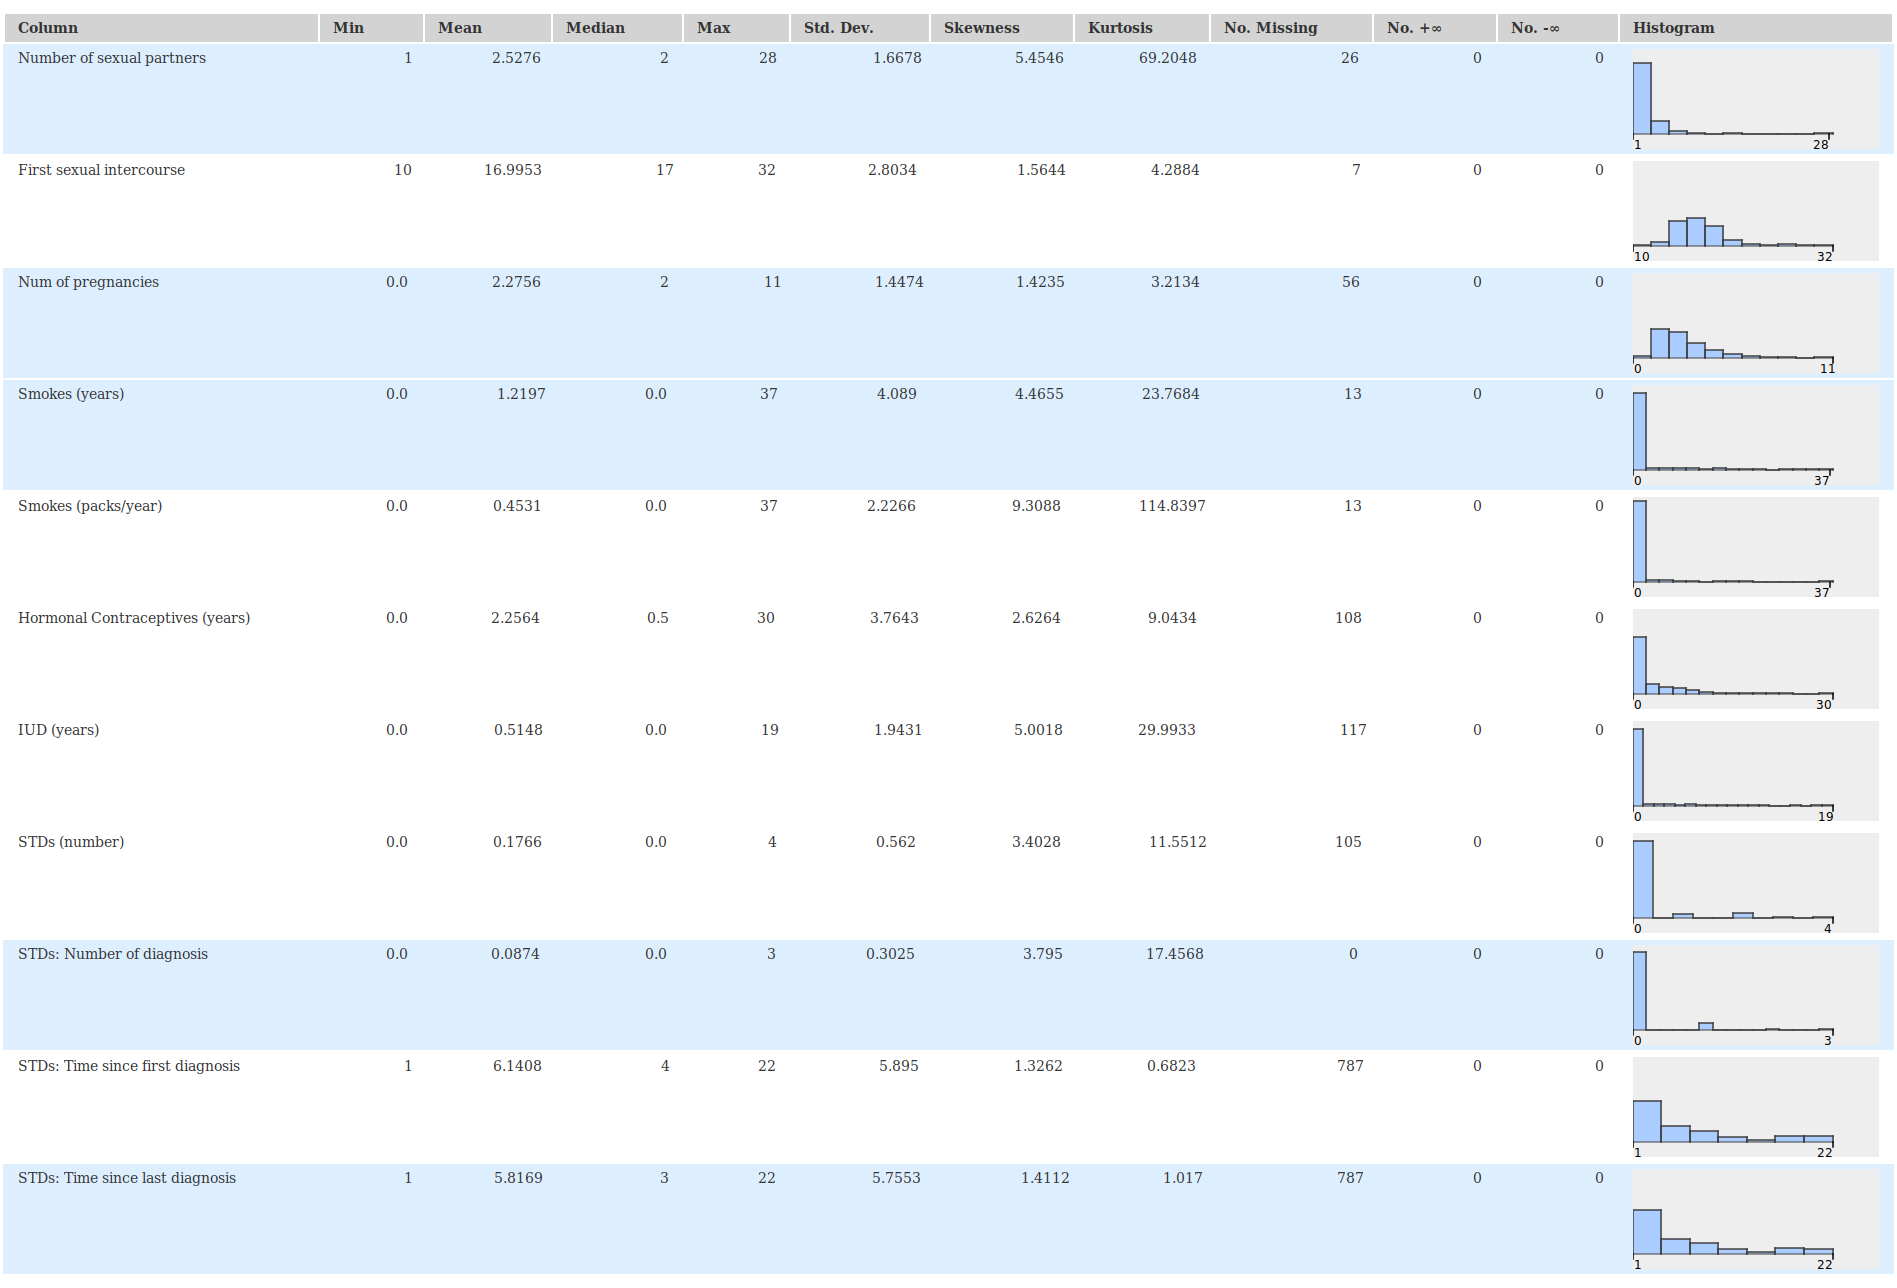
\includegraphics[width=0.95\paperwidth]{figures/numeric_statistics.pdf}}
    \caption{Numeric attributes statistics}
    \label{numeric_attributes_statistics}
\end{figure}

\begin{figure}[H]
    \centerline{
        \includegraphics[width=0.9\paperwidth]{figures/scatter.png}}
    \caption{Scatter Matrix of Age, Number of sexual partners, First sexual intercourse, Biopsy}
    \label{scatter}
\end{figure}

\end{document}